\documentclass[lang=cn, chinesefont=founder, color=cyan, citestyle=gb7714-2015, bibstyle=gb7714-2015]{elegantbook}

\usepackage{unicode-math}
\setmathfont{STIXTwoMath-Regular.otf}

\usepackage[color=black]{siunitx}
\usepackage{tikz}
\usepackage{tkz-euclide}
\usepackage{tkz-graph}
\usepackage{dashrule}
\PassOptionsToPackage{dvipsnames,svgnames,x11names}{xcolor}

\definecolor{shadow}{RGB}{210,241,241}

\newcommand{\spare}{\vspace{-1em}\begin{center}\color{structurecolor}\hdashrule[0.5ex]{\textwidth}{1pt}{1pt}\end{center}\vspace{-1em}}
\usetikzlibrary{shapes,backgrounds}
\ExecuteBibliographyOptions{sorting=gb7714-2015}
\setlength{\parskip}{1ex}
\newtcolorbox{collections}{
      boxrule=0.5pt,
      enhanced,
      breakable,
      top=8pt,
      before skip=8pt,
      colframe=structurecolor,
      colback=structurecolor!5,
      colbacktitle=structurecolor
}
\renewcommand{\bar}[1]{\overline{#1}}
\renewcommand\arraystretch{1.3}
\arrayrulecolor{second}

\usetikzlibrary{graphs}

\title{新世代计算机科学计划·基础篇}
\author{JouderMin}
\institute{「新世代计算机科学计划」制作委员会}
\date{\zhtoday}
\cover{img/cover.png}
\logo{img/方形logo.png}

\begin{document}
\maketitle
\frontmatter

\tableofcontents

\mainmatter

\chapter{离散数学}
\input{SectionPage/1.1.tex}
\input{SectionPage/1.2.tex}

\section{图的概念}
\begin{introduction}
    \item 图
    \item 无向图、有向图与混合图
    \item 环、多重边
    \item 简单图、伪图与多重图
    \item 顶点与边的性质
\end{introduction}

\subsection{图}
图是由顶点与连接顶点的边构成的离散结构,图的定义如下
\begin{definition}[图]\label{def:图}
    图 $G = (V, E)$ 由顶点的非空集 $V$ 和边集 $E$ 构成,每条边有一个或两个顶点与之相连,这样的顶点叫做边的端点。
\end{definition}

图 \ref{fig:图} 展示了一个图。
\begin{figure}[htbp!]
    \centering
    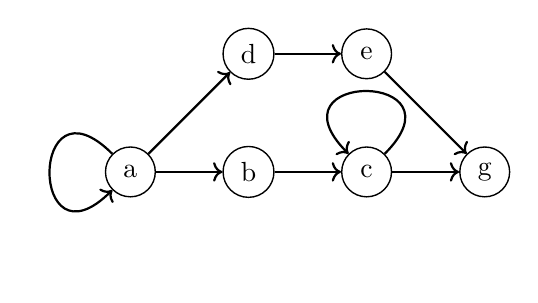
\begin{tikzpicture}
        \GraphInit[vstyle=normal]
        \SetGraphUnit{1.5}
        \Vertex{a}
        \EA(a){b}
        \EA(b){c}
        \EA(c){g}
        \NO(b){d}
        \NO(c){e}
        \Edge[style={->}](a)(b)
        \Edge[style={->}](b)(c)
        \Edge[style={->}](c)(g)
        \Edge[style={->}](a)(d)
        \Edge[style={->}](d)(e)
        \Edge[style={->}](e)(g)
        \Loop[dist=1.5cm, style={->}](a)
        \Loop[dist=1.5cm, dir=NO, style={->}](c)
    \end{tikzpicture}
    \caption{图}
    \label{fig:图}
\end{figure}

\subsection{无向图、有向图与混合图}
图可以根据边是否有方向这一特性来划分为无向图、有向图与混合图三类。
\begin{definition}[有向边与无向边]\label{def:无向边与有向边}
    无向边以基数为 2 的集合表示,$\{u, v\}$ 表示该无向边与顶点 $u$、$v$ 相关联。有向边以序偶表示,$(u, v)$ 表示该有向边与顶点 $u$、$v$ 相关联,且开始于 $u$,结束于 $v$。
\end{definition}

由此,如果图 $G$ 的边集 $E$ 中只有无向边,则该图称为无向图;如果图 $G$ 的边集 $E$ 中只有有向边,则该图称为有向图;如果图 $G$ 的边集 $E$ 中同时存在无向边与有向边,则该图称为混合图。
\begin{figure}[htbp!]
    \centering
    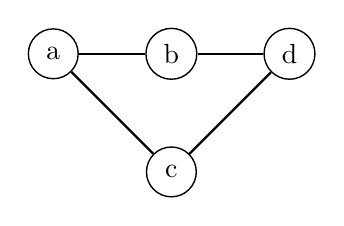
\begin{tikzpicture}
        \GraphInit[vstyle=normal]
        \SetGraphUnit{1.5}
        \Vertex{a}
        \EA(a){b}
        \SO(b){c}
        \EA(b){d}
        \Edge[style={-}](a)(b)
        \Edge[style={-}](a)(c)
        \Edge[style={-}](b)(d)
        \Edge[style={-}](c)(d)
    \end{tikzpicture}
    \hspace{1em}
    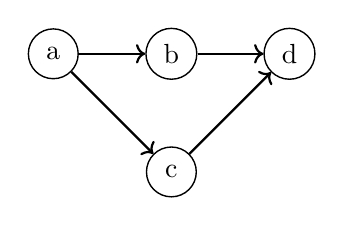
\begin{tikzpicture}
        \GraphInit[vstyle=normal]
        \SetGraphUnit{1.5}
        \Vertex{a}
        \EA(a){b}
        \SO(b){c}
        \EA(b){d}
        \Edge[style={->}](a)(b)
        \Edge[style={->}](a)(c)
        \Edge[style={->}](b)(d)
        \Edge[style={->}](c)(d)
    \end{tikzpicture}
    \hspace{1em}
    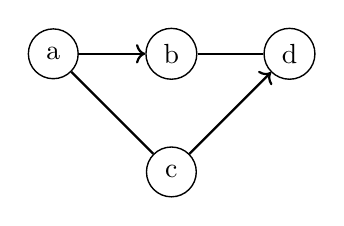
\begin{tikzpicture}
        \GraphInit[vstyle=normal]
        \SetGraphUnit{1.5}
        \Vertex{a}
        \EA(a){b}
        \SO(b){c}
        \EA(b){d}
        \Edge[style={->}](a)(b)
        \Edge[style={-}](a)(c)
        \Edge[style={-}](b)(d)
        \Edge[style={->}](c)(d)
    \end{tikzpicture}
    \caption{无向图(左)、有向图(中)、混合图(右)}
\end{figure}

\subsection{环、多重边、简单图、伪图与多重图}
如果一条边所连接的顶点是同一个顶点,那么该边称为环。如果多条边连接同一对顶点,那么称其为多重边。
\begin{figure}[htbp!]
    \centering
    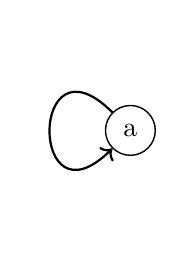
\begin{tikzpicture}
        \GraphInit[vstyle=normal]
        \SetGraphUnit{1.5}
        \Vertex{a}
        \Loop[dist=1.5cm, style={->}](a)
    \end{tikzpicture}
    \hspace{1em}

    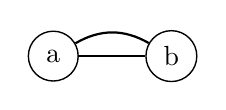
\begin{tikzpicture}
        \GraphInit[vstyle=normal]
        \SetGraphUnit{1.5}
        \Vertex{a}
        \EA(a){b}
        \Edge[style={-, bend left}](a)(b)
        \Edge[style={-}](a)(b)
    \end{tikzpicture}
    \caption{环(上)与多重边(下)}
    \label{fig:环与多重边}
\end{figure}

如果一个图不存在多重边或者环,那么该图被称为简单图;如果一个图存在多重边和环,那么该图被称为伪图;如果一个图存在多重边但不存在环,那么该图称为多重图。

\begin{table}[htbp!]
    \centering
    \begin{tabular}{ccc}
        \toprule
        \makebox[2cm][c]{多重边} & \makebox[2cm][c]{环} & \makebox[2cm][c]{类型} \\
        \midrule
        不存在 & 不存在 & 简单图 \\
        存在 & 存在 & 伪图 \\
        存在 & 不存在 & 多重图 \\
        \bottomrule
    \end{tabular}
    \caption{简单图、伪图与多重图}
\end{table}

\begin{figure}[htbp!]
    \centering
    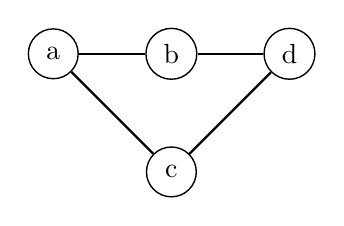
\begin{tikzpicture}
        \GraphInit[vstyle=normal]
        \SetGraphUnit{1.5}
        \Vertex{a}
        \EA(a){b}
        \SO(b){c}
        \EA(b){d}
        \Edge[style={-}](a)(b)
        \Edge[style={-}](a)(c)
        \Edge[style={-}](b)(d)
        \Edge[style={-}](c)(d)
    \end{tikzpicture}
    \hspace{1em}
    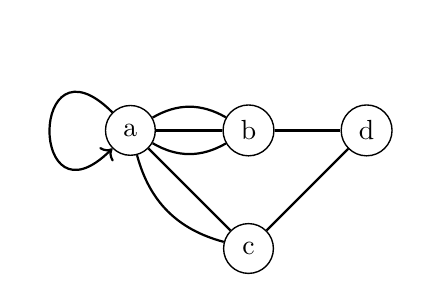
\begin{tikzpicture}
        \GraphInit[vstyle=normal]
        \SetGraphUnit{1.5}
        \Vertex{a}
        \EA(a){b}
        \SO(b){c}
        \EA(b){d}
        \Edge[style={-}](a)(b)
        \Edge[style={-, bend left}](a)(b)
        \Edge[style={-, bend right}](a)(b)
        \Edge[style={-, bend right}](a)(c)
        \Edge[style={-}](a)(c)
        \Edge[style={-}](b)(d)
        \Edge[style={-}](c)(d)
        \Loop[dist=1.5cm, style={->}](a)
    \end{tikzpicture}
    \hspace{1em}
    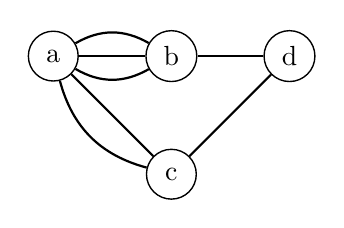
\begin{tikzpicture}
        \GraphInit[vstyle=normal]
        \SetGraphUnit{1.5}
        \Vertex{a}
        \EA(a){b}
        \SO(b){c}
        \EA(b){d}
        \Edge[style={-}](a)(b)
        \Edge[style={-, bend left}](a)(b)
        \Edge[style={-, bend right}](a)(b)
        \Edge[style={-, bend right}](a)(c)
        \Edge[style={-}](a)(c)
        \Edge[style={-}](b)(d)
        \Edge[style={-}](c)(d)
    \end{tikzpicture}
    \caption{简单图(左)、伪图(中)、多重图(右)}
\end{figure}

\subsection{顶点与边的性质}
\begin{definition}[无向图顶点的邻接]\label{def:无向图邻接}
    若 $u$ 和 $v$ 是无向图 $G$ 中的一条边 $e$ 的端点,则称两个顶点 $u$ 和 $v$ 在 $G$ 里邻接,边 $e$ 关联(或连接)$u$ 和 $v$
\end{definition}
\begin{definition}[有向图顶点的邻接]\label{def:有向图邻接}
    若 $(u,v)$ 是有向图 $G$ 中的一条边,则称顶点 $u$ 邻接到 $v$,$v$ 从 $u$ 邻接,$u$ 称为边 $(u,v)$ 的起点,$v$ 称为边 $(u,v)$ 的终点。环的起点与终点相同。
\end{definition}
\begin{definition}[顶点的邻居]\label{def:邻居}
    图 $G=(V, E)$ 中,顶点 $v$ 的所有邻接顶点的集合称为顶点的邻居,记作 $N(v)$。
\end{definition}

\begin{collections}
    \begin{example}
        写出下图中各个顶点的邻居。
            \begin{center}
                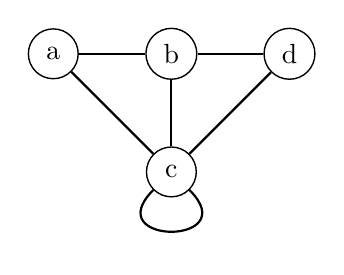
\begin{tikzpicture}
                    \GraphInit[vstyle=normal]
                    \SetGraphUnit{1.5}
                    \Vertex{a}
                    \EA(a){b}
                    \SO(b){c}
                    \EA(b){d}
                    \Edge[style={-}](a)(b)
                    \Edge[style={-}](a)(c)
                    \Edge[style={-}](b)(d)
                    \Edge[style={-}](c)(d)
                    \Edge[style={-}](b)(c)
                    \Loop[dist=1cm, style={-}, dir=SO](c)
                \end{tikzpicture}
            \end{center}
    \end{example}
    \begin{solution}
        \begin{center}
            \begin{tabular}{c|c}
                \toprule
                \makebox[2cm][c]{顶点} & \makebox[2cm][c]{邻居} \\
                \midrule
                a & b, c \\
                b & a, c, d \\
                c & a, b, c, d \\
                d & b, c \\
                \bottomrule
            \end{tabular}
        \end{center}

    \end{solution}
\end{collections}

\begin{definition}[无向图顶点的度]
    无向图中顶点的度是与该顶点相关联的边的数目,如果该顶点存在环,则每个环为顶点的度贡献 2。顶点 $v$ 的度记作 $\symrm{deg}(v)$
\end{definition}

\end{document}